\documentclass{article}

% For HTML output
%\def\pgfsysdriver{pgfsys-tex4ht.def} 

\usepackage[a4paper]{geometry}
\usepackage{charter}
\usepackage{tikz}
\usepackage{array}
\usepackage{natbib}
\usetikzlibrary{automata}

\title{Tracter}
\author{Philip N. Garner}

\begin{document}

\maketitle
\tableofcontents

\begin{abstract}
  This is currently a rather disconnected set of ramblings about
  tracter.  One day it will be a user manual.  One day.
\end{abstract}

\section{Introduction}
\subsection{Overview}

Tracter is a data-flow framework for signal processing.  It defines a
library of components that each typically do a small amount of
computation, but can become nodes in a directed graph where they work
together (although independently) to do something more useful.

Although tracter contains several implementations of basic algorithms,
it has developed into a wrapper for libraries of basic algorithms.

The components generally run serially, not in parallel; tracter does
not do concurrent data-flow in the sense of Kahn process networks
\citep{Lee1995}.

Tracter distinguishes sources and sinks.

%\begin{tikzpicture}[start chain]
%  \node [draw,on chain] {A};
%  \node [draw,on chain] {B};
%  \node [draw,on chain] {C};
%\end{tikzpicture}

\subsection{API}

One of the packages I use to write this document is called TikZ.  TikZ
is an astounding piece of software; I had no idea it was possible to
do things like that in \TeX.  However, the reason I mention it here is
that I think it has a very nicely designed API.  Tikz has 3 distinct
levels:
\begin{description}
\item[TikZ] itself is a top level interface to PGF.
\item[PGF] is the actual language.
\item[The underlying driver] layer disconnects PGF from the means of
  rendering the graphics.
\end{description}
For me, tikz is an example of a really well thought out API.  It's
well documented too - just the table of contents is 13 pages.

Tracter aims to have this sort of hierarchical API.  I'm not sure it
really succeeds, but the idea is to have about 4 or 5 layers:
\begin{description}
\item[Executables] are the top layer.  Generally speaking it's
  possible to write an executable that has just one tracter component
  and does something useful.
\item[Factories] are the same level as some other APIs.  They define a
  graph of components that constitute some useful block.  A factory is
  actually a very thin layer; it just instantiates a graph of
  components, so the overhead afer calling the factory is zero.
\item[Components] are the main level.  A component is a node in a
  directed graph of processing elements.  Components necessarily have
  inputs and outputs.  To use them you have to buy into the data-flow
  idea.
\item[Objects] in tracter are things that have a name and can hence
  receive parameters.  They don't necessarily take part in data flow
  operations.  Factories are objects, as are components.
\item[Algorithms] are the bottom layer; fundamental functions.  These
  are the sorts of things that BLAS and LAPACK provide, and also
  comprise DFTs, filters and the like.  They might even be written in
  C or FORTRAN; not necessarily C++.
\end{description}

The most important level in tracter is the component
level.\footnote{At the time of writing, this is the plugin level.  But
  plugin is a bad name; it implies dynamic loading, which is not what
  tracter is about.}  It is possible to write only components.
However, if a component is really useful, it tends to be desirable to
break it down into other objects, but objects that still require
parameters to be passed to them.

Tracter is really the wrong place to put fundamental functions.  Those
belong in other libraries because they are useful outside the scope of
tracter.

An example of the hierarchy is a frequency warp.  It is possible to
write a program that has a small number of components that calculate a
frequency warp; the input is a periodogram and the output is a file,
or cepstrum or the like.  In this sense, the warp is a component in
the data-flow.  The frequency warp component itself is really just a
fundamental function.  However, it has a lot of parameters, and can be
used in different situations; this is an object in tracter terms.
Ultimately, however, the frequency warp is a function with parameters
that may even be implemented in some third party library; IPP for
instance.

This idea of fundamental libraries is one key point of tracter,
completely independent from the data-flow part.  It brings together
many independent libraries and allows them to be used in the same
framework.  This is not a new thing; Octave does it, as does MPlayer.

Somewhere in there is an interface layer too.  The idea that you can
have alternative implementations of the same functionality.  Typically
this is a DFT that could be from Kiss FFT, FFTW or even IPP.

There is a programming methodology called ``Extreme Progamming'' (EP).
EP encompasses many different philosophies, but one of them is the
idea that you should implement only as much as you need.\footnote{In
  some sense, tracter is way too over-engineered.}  The way to apply
EP in tracter is to first write a technique as a component.  If the
component is useful, expand it into one or more objects that are
contained by a component.  If the core algorithms are useful, they can
be abstracted out as a fundamental functions.

That said, most of the fundamental functions are already written and
exist in other libraries.  In this sense, tracter reduces to an
exercise in writing Gnu configure scripts.


%%% Local Variables: 
%%% mode: latex
%%% TeX-master: "tracter"
%%% TeX-PDF-mode: t
%%% End: 

\section{Segmenter behaviour}

\subsection{VAD}

Whatever feature the VAD uses, it ultimately drives a state machine
with four states as illustrated in figure \ref{fig:StateMachine}.  The
purpose of the state machine is to place minimum time limits on speech
and silence segments.
\begin{figure}[htb]
  \centering
  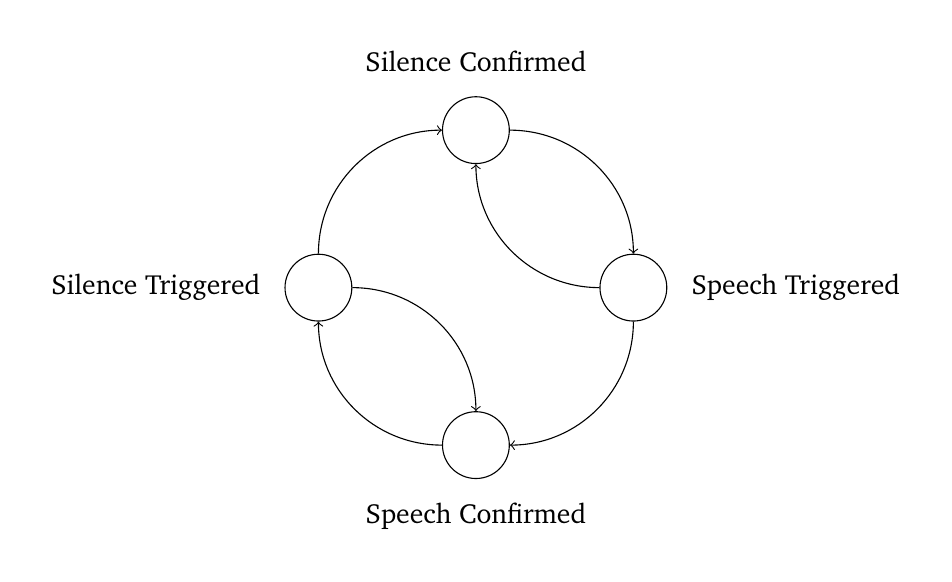
\begin{tikzpicture}
    [inner sep=3mm,state/.style={circle,draw=black}]
    \node (silconf) at (0,2)  [state] {};
    \node (spetrig) at (2,0)  [state] {};
    \node (speconf) at (0,-2) [state] {};
    \node (siltrig) at (-2,0) [state] {};
    \node [above] at (silconf.north) {Silence Confirmed};
    \node [right] at (spetrig.east)  {Speech Triggered};
    \node [below] at (speconf.south) {Speech Confirmed};
    \node [left]  at (siltrig.west)  {Silence Triggered};
    \draw [->] (silconf) to [out=0,in=90]  (spetrig);
    \draw [->] (spetrig) to [out=-90,in=0] (speconf);
    \draw [->] (speconf) to [out=180,in=-90] (siltrig);
    \draw [->] (siltrig) to [out=90,in=180] (silconf);
    \draw [->] (spetrig) to [out=180,in=-90] (silconf);
    \draw [->] (siltrig) to [out=0,in=90] (speconf);
  \end{tikzpicture}
  \caption{VAD state machine}
  \label{fig:StateMachine}
\end{figure}

The state machine always begins in state ``Silence Confirmed'' and
moves to state ``Speech Triggered'' on voice activity.  If voice
activity remains for at least time $t_V$ then the state machine
progresses to state ``Speech confirmed'', otherwise it moves back to
``Silence Confirmed''.  A similar process governs the left hand half
of the state machine, depending on $t_S$, a time for silence
detection.  This is further illustrated in figure
\ref{fig:StateLevel}.
\begin{figure}[htb]
  \centering
  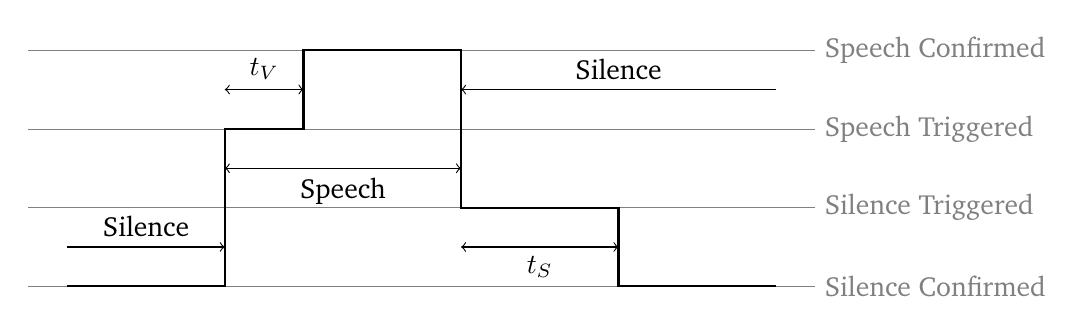
\begin{tikzpicture}
    \draw [help lines] (-.5,0) -- (9.5,0) node [right] {Silence Confirmed};
    \draw [help lines] (-.5,1) -- (9.5,1) node [right] {Silence Triggered};
    \draw [help lines] (-.5,2) -- (9.5,2) node [right] {Speech Triggered};
    \draw [help lines] (-.5,3) -- (9.5,3) node [right] {Speech Confirmed};
    \draw [thick] (0,0)
    -- (2,0)
    -- (2,2) -- (3,2)
    -- (3,3) -- (5,3)
    -- (5,1) -- (7,1)
    -- (7,0) -- (9,0);
    \draw [<->] (2,1.5) -- node [auto,swap] {Speech} (5,1.5);
    \draw [<->] (2,2.5) -- node [auto] {$t_V$} (3,2.5);
    \draw [<->] (5,0.5) -- node [auto,swap] {$t_S$} (7,0.5);
    \draw [->] (0,0.5) -- node [auto] {Silence} (2,0.5);
    \draw [<-] (5,2.5) -- node [auto] {Silence} (9,2.5);
  \end{tikzpicture}
  \caption{State level diagram for VAD.  Left to right dimension is
    time.}
  \label{fig:StateLevel}
\end{figure}


\subsection{Data flow}

Tracter components respond to fetch operations from the output caches.
The fetch will ask a component for a particular number of frames, $N$,
and the component should request enough data from its input components
to supply those $N$ frames.  The source components should block until
enough data become available.  The fetch operation should then return
an integer corresponding to the number of frames that were written to
the cache; this is normally $N$.

When data are no longer available, the components should return a
number less than $N$.  Such a case is always indicative of data flow
having been interrupted.  This is the only signal that a component is
able to send downstream to indicate that data is no longer available.
Call this the End Of Data signal (EOD).

Downstream components will typically simply pass on EOD by returning
frame counts less than those that were requested.  Some may choose to
take some ``edge effect'' action, duplicating the final frame for
instance, but will always eventually pass on EOD.

Depending upon the application, a sink component can restart data flow
by sending a reset signal.  This can be done, for instance, after
changing a file-name at the source.  Reset does not close connections;
it just resets counters and empties caches.

A (VAD) gate component is special because it can choose to block
reset.  When the end of a (speech) segment is detected, the gate
returns EOD.  The application then resets the flow graph and requests
more data.  Instead of propagating the reset upstream, the gate blocks
it and simply restarts data flow at the beginning of the next segment.
The gate component hence introduces extra EOD signals corresponding to
end of segment.  The application does not know the difference between
a real EOD and the fake EOD generated by the gate.

We have identified four different ``modes'' for the VAD gate in the
context of an application:
\begin{description}
\item[Offline] In offline mode, the input is typically a file.  The
  file is assumed to contain only one segment; the end of the segment
  is taken to be the end of the file.  The application resets after
  the segment; reset is likely to be accompanied by the application
  changing the file-name on the source.
\item[Offline segmented] As offline, but the file is assumed to
  contain several segments.  Reset should simply move to the next
  segment.  However, the end of the file is then difficult to spot.
  The VAD gate is aware of EOF because upstream components will
  indicate end of data.  The VAD gate indicates this to the
  application by returning 0 frames for the first fetch after the end
  of the file.  We call this a double EOD.
\item[Online] Online is taken to mean that the input is ``live'' in
  some sense.  The VAD gate is acting as a segmenter, and reset is
  taken to mean select the next segment.  The real end of data implies
  part of the system has shut-down.
\item[PTT] Push To Talk.  The data is online, but is being segmented
  to an extent by user intervention.  The end of data does not
  correspond to a shut-down; it just means that the application should
  wait until more data arrives.
\end{description}

\begin{table}[htb]
  \centering
  \begin{tabular}{|m{2cm}|m{3cm}|m{3cm}|m{3cm}|}
    \hline
    {\bf Mode} & {\bf Source} & {\bf Gate} & {\bf Sink / Application} \\
    \hline\hline
    Offline
    & EOD at EOF
    & Propagate reset
    & Reset after EOD, change file \\
    \hline
    Offline segmented
    & EOD at EOF
    & Block reset, propagate after EOD
    & Reset after EOD, change file after double EOD \\
    \hline
    Online
    & EOD at shut-down
    & Block reset
    & Shut-down after EOD \\
    \hline
    PTT
    & EOD at each segment
    & Propagate reset
    & Reset after EOD \\
    \hline
  \end{tabular}
  \caption{Mapping of segmentation modes to component behaviour.}
  \label{tab:SegmentationMode}
\end{table}

Table \ref{tab:SegmentationMode} shows the mapping between these modes
and behaviour of the source, gate and sink components.  Notice that:
\begin{enumerate}
\item The source really only has one mode: EOD is sent whenever it
  detects the end of a segment.
\item The gate has three modes, but given that the sink will never
  respond to a double EOD in online mode, it can be thought of as just
  two.  It doesn't care about whether it is online or offline, rather
  it needs to know whether to segment continuously or not.
\item The sink needs to be able to detect double EOD for the offline
  segmented mode.  However, given that it will only receive double EOD
  in that mode, it need not distinguish the special case.
\end{enumerate}


\subsection{Special cases}

The diagrams in figures \ref{fig:StateMachine} and
\ref{fig:StateLevel} are somewhat idealistic.  There are two
degenerate cases in particular that occur regularly, especially in
Offline and PTT modes:
\begin{enumerate}
\item No segment exists before EOF.
\item A segment begins but does not end before EOF.
\end{enumerate}
In the first case, the gate detects no signal at all and remains in
state ``Silence confirmed''.  In the second, the gate detects the
beginning of a signal, but not the end.


\subsection{Silence removal}

There is one more mode that is not mentioned above - Silence removal.
In this mode, silence between words is removed.  Without true
continuous speech recognition, this can only really work in cases
where there is another more persuasive utterance end indicator, i.e.,
the end of a file or a push-to-talk switch.




%%% Local Variables: 
%%% mode: latex
%%% TeX-master: "tracter"
%%% TeX-PDF-mode: t
%%% End: 

\section{Framing}

Framing is the process of taking a data stream and reading a frame (or
window) of data rather than a single datum.  Further processing is
then done on the frame rather than the individual data.  In fact,
tracter refers to all data as frames; this is a precedent taken from
ALSA.

\begin{figure}[htb]
  \centering
  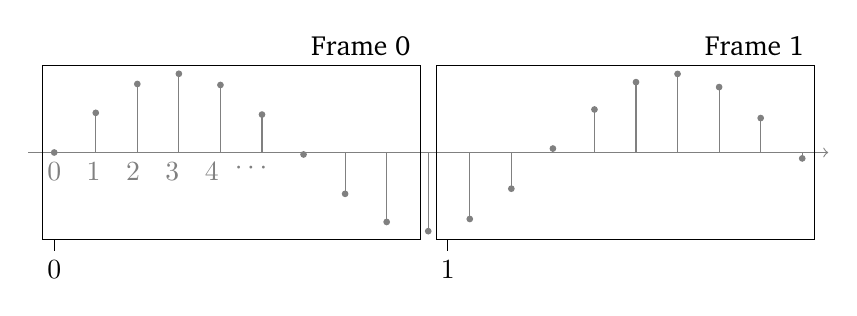
\begin{tikzpicture}[scale=.5,domain=0:19,samples=19]
    \draw[gray,->] (-.66,0) -- (19.66,0);
    \draw[gray] plot[ycomb,mark=*] (\x, {2*sin(\x r/2)});
    \foreach \x in {0,...,4} \draw (\x,0) node [gray, below] {$\x$};
    \draw (5,0) node [gray, below] {$\cdots$};
    \draw (-.3,-2.2) rectangle (9.3,2.2) node [above left] {Frame 0};
    \draw (9.7,-2.2) rectangle (19.3,2.2) node [above left] {Frame 1};
    \draw (0,-2.2) -- (0,-2.5) node [below] {$0$};
    \draw (10,-2.2) -- (10,-2.5) node [below] {$1$};
  \end{tikzpicture}
  \caption{Frame indexing is aligned with the first sub-frame within
    each frame.  Framing components hence look ahead in time.}
  \label{fig:Frame}
\end{figure}

By convention, the frame index is assumed to be aligned with that of
the first component frame, as illustrated in figure \ref{fig:Frame}.
This means that framing components look ahead in time.  This in turn
has to be indicated in the {\tt MinSize()} call.


\begin{figure}[htb]
  \centering
  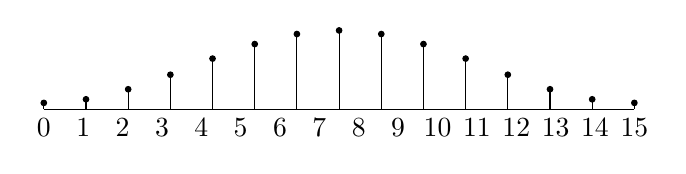
\begin{tikzpicture}[scale=.5,domain=0:15,samples=15]
    \draw (0,0) -- (15,0);
    \foreach \x in {0,...,15} \draw (\x,0) node [below] {$\x$};
    \draw plot[ycomb, mark=*] (\x, {2*(.54 - .46 * cos(360*\x/15))});
  \end{tikzpicture}
  \caption{Hamming window
    $f(x)=0.54-0.46\cos\left(2\pi\frac{x}{N-1}\right)$ with $N=16$}
  \label{fig:Hamming}
\end{figure}


\begin{figure}
  \centering
  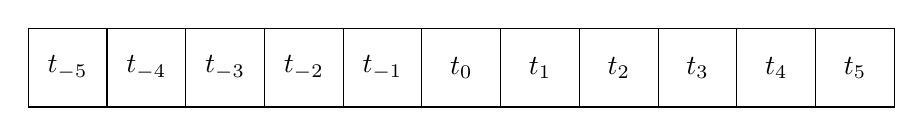
\begin{tikzpicture}
    \foreach \x in {-5,...,5}
    {
      \draw (\x,0) +(-.5,-.5) rectangle ++(.5,.5);
      \draw (\x,0) node{$t_{\x}$};
    }
  \end{tikzpicture}
  \caption{Useful looking boxes in a row.}
\end{figure}

%%% Local Variables: 
%%% mode: latex
%%% TeX-master: "tracter"
%%% TeX-PDF-mode: t
%%% End: 


\bibliographystyle{plainnat}
\bibliography{phil-refs}

\end{document}

%%% Local Variables: 
%%% mode: latex
%%% TeX-master: t
%%% TeX-PDF-mode: t
%%% End: 
